\documentclass[compress,xcolor={dvipsnames}]{beamer}
\usepackage{fancyvrb,newverbs} % For customized verbatim
\usepackage{calligra} % A fancy text for ending `Thank you'
\usepackage[T1]{fontenc}
\usefonttheme[onlymath]{serif}

\author{Zihang Wang}
\title{Phase Field Tutorial}
\subtitle{C++ Programming and Calculation Examples}
\institute{Central South University}

\AtBeginSubsection[]
{
	\begin{frame}
		\tableofcontents[sectionstyle=show/shaded,subsectionstyle=show/shaded/hide,subsubsectionstyle=show/shaded/hide]
	\end{frame}
}
\usetheme{Berlin}

\setbeamertemplate{footline} {
    \begin{beamercolorbox}[ht=2.5ex,dp=1.125ex,
      leftskip=.3cm,rightskip=.3cm plus1fil]{title in head/foot}
      {\usebeamerfont{institute in head/foot}\usebeamercolor[fg]{institute in head/foot}\insertshortinstitute}
      \hfill
      {\centering\usebeamerfont{title in head/foot}\insertshortsubtitle}
      \hfill
      {\usebeamerfont{frame number}\usebeamercolor[fg]{frame number}\insertframenumber~/~\inserttotalframenumber}
    \end{beamercolorbox}
    \begin{beamercolorbox}[colsep=1.5pt]{lower separation line foot}
    \end{beamercolorbox}
}

% ---------------------------------------------------------------------------
\definecolor{cverbbg}{gray}{0.93}

\newenvironment{cverbatim}
 {\SaveVerbatim{cverb}}
 {\endSaveVerbatim
  \flushleft\fboxrule=0pt\fboxsep=.5em
  \colorbox{cverbbg}{\BUseVerbatim{cverb}}%
  \endflushleft
}
\newenvironment{lcverbatim}
 {\SaveVerbatim{cverb}}
 {\endSaveVerbatim
  \flushleft\fboxrule=0pt\fboxsep=.5em
  \colorbox{cverbbg}{%
    \makebox[\dimexpr\linewidth-2\fboxsep][l]{\BUseVerbatim{cverb}}%
  }
  \endflushleft
}
\newverbcommand{\cverb}
  {\setbox\verbbox\hbox\bgroup}
  {\egroup\colorbox{cverbbg}{\box\verbbox}}

\setlength{\parindent}{2em}

\newcommand{\bhref}[2]{
    \href{#1}{\color{blue}{#2}}
}
% ---------------------------------------------------------------------------

\begin{document}
\begin{frame}
    \titlepage
    \begin{figure}[!h]
        \centering
        
\includegraphics[width=0.18\linewidth]{pic/csulogo.jpg}
        
\includegraphics[width=0.25\linewidth]{pic/MInDes_Icon.jpg}
    \end{figure}
\end{frame}

\begin{frame}
    \tableofcontents[currentsection, hideothersubsections, sectionstyle=show/show]
\end{frame}

% ---------------------------------------------------------------------------
\section{Review \& Intro}
\begin{frame}
    \frametitle{Quick Review}
    What have we got in the last tutorial?

    \begin{itemize}
        \item Python Installation
        \item Programming Basics (Python)
        \item Forward / Backward Euler Method
        \item OOP and Numerical Integral
        \item OOP and Gradient \& Laplacian
    \end{itemize}

    While, with these numerical methods implemented with Python, Let's try to combine them together, with \emph{C++}.
\end{frame}

\begin{frame}
    \frametitle{C++, a `better C' }
    C++, a programming language designed by Bjarne Stroustrup in 1979, was originally designed to be an improved C, has
    become one of the most popular programming languages in the world. It supports OOP, template programming, and many otehr
    useful features. It's so efficient that can be compared with C. All these features enabling it to be an
    ideal choice for scientific computation.
    \bigbreak
    \pause
    However, it is also a complicated language There are messive details of grammar, and some features
    make it not so friendly to programmers. Some common things in other language could be not that easy in C++.
    \bigbreak
    \pause
    But, fortunately, to learn and do some calculation with C++, all you need is almost there.
\end{frame}

\begin{frame}
    \frametitle{What's our plan?}
    So, where shall we start from? What shall we do? Repeat the algorithm in the last tutorial, and just implement them in C++?
    \bigbreak
    \pause
    That's half-right. We won't cover all details in implementing these algorithm. What we are going to do are:
    \begin{enumerate}
        \item C++ Environment Setup;
        \item C++ vs Python: Language Grammar \&  Features;
        \item Something Familar: Integration;
        \item Simple Example: 1D Transient Heat Conduction.
    \end{enumerate}
    \pause
    That's a lot. Let's start our very first step: environment setup.
\end{frame}

% ---------------------------------------------------------------------------
\section{Setup Your Environment}
\subsection{Before we start}
\begin{frame}
    \frametitle{Make a Choice}
    Okay, you must can't wait to download something. But there are bunch of choices, and some of you might
    end up with wrong configuration, frustrated and stay away from C++ to retain your mental health. So to save your time,
    I recommend three way to get started with C++:
    \pause
    \begin{itemize}
        \item The newest Visual Studio Community Edition if you are runing on Windows.
        \item The GCC compiler tool chain chain with Linux or WSL if you are on Linux or want to give it a try.
        \item The Clang/LLVM compiler tool chain if you are on Mac OS or you just don't like the former two.
    \end{itemize}
    \pause
    Let's see what are they and their features.
\end{frame}
\begin{frame}[fragile]
    \frametitle{VS: The Best IDE for Windows C++ Dev (Maybe\footnote{There are still many other choice, and everyone has their own choice, too. For me myself, VS is good.})}
    Visual Studio (abbr. as \emph{VS}), an IDE from Microsoft for developing C++ or .Net on Windows, usually is the best choice for any C++ programmer
    using Windows. As an IDE, VS is fully equipped with editor, linter, compiler, debugger and analyzer. After some \emph{right} clicks, you are then ready for C++ progrmming, and just skip the tiring prerequisite. You can focus yourself on programming and solving problems.
    \pause

    However, there are flaws in VS. VS is a \emph{BIG} software needing a lot of drive space to install it. And, some components must be installed under your \cverb|C| drive. But if that's okay for you, VS should be the first choice.
\end{frame}

\begin{frame}[fragile]
    \frametitle{GCC: Old, but powerful.}
    Well, if you are not a Windows user, or want to compile C++ for other platform, or just don't want to use VS and MSVC (Compiler used by VS), Then you can try GCC, the GNU Compiler Collection.
    \pause

    What is GNU? GNU is Not Unix! That will be a long story to tell about GNU, Linux, GCC and open source software. But if you are going to write your code on Linux, your first choice will always be GCC tool chain, explicitly, \cverb|g++|, \cverb|gdb| and \cverb|makefile|, which are compiler, debugger and build system, respectively. All of these tools have long histories, but are powerful and never outdated.
    \pause

    If you are interested in GCC and Linux, but already a Windows user, I recommend you to install `WSL' on your Windows. That will give you almost the original experience of a Linux system.
\end{frame}

\begin{frame}
    \frametitle{Clang/LLVM: Progressive New Force}
    If you are on Mac OS, after install gcc and check your installation, you will be surprised by prompt from `Clang'. That's because Mac OS use Clang/LLVM as its default C/C++ compiler.
    \pause

    Clang is a part of LLVM Project, which is originally a research project at University of Illinois. Clang is a compiler that compatible with many backends, such as MSVC and GCC. And, as a fully modularized compiler, it has a great potential to be extended and developed, and is a good example for whom studying compiler theory and language design.
    \pause

    Well, we don't actually need to learn compiler or language design. What's good for choosing Clang? If you are using Mac OS, that will be your first choice. Or you can just give it a try. Clang is famous for its readable and helpful error/warn messages. Maybe you will like it.
\end{frame}
\subsection{Set It Up!}
\begin{frame}[fragile]
    \frametitle{Let's do it}

    By now you should have made your choice. Let's start to set our enviornment up.
    \pause

    If you choose to install Visual Studio from Microsoft, please download the installer (yes, you need install the installer first), and \emph{select `Desktop development with C++'}. Then you can just accept the default settings.
    \pause

    If you choose to install WSL and GNU, I recommend reading WSL guide from Microsoft before install it, and installing VS Code. VS Code has good support to WSL and C++ programming with extension. Then after WSL setup, you can install GNU tool chain by \cverb|sudo apt install build-essential|.
    \pause

    If you are using Mac OS, you can use \cverb|homebrew| to install Clang, and choose your favourite editor or IDE.

\end{frame}

\begin{frame}[fragile]
    \frametitle{Your First C++ Code}

    So, let's try to write a little piece of C++ code.

    Your first C++ code, as usual, will be a simple `Hello World':
    \begin{lcverbatim}
        #include <iostream>

        int main(){
                std::cout<< "Hello C++ World!\n";
        }
    \end{lcverbatim}
    This code includes many points. You use \cverb|#include| to \emph{Copy \& Paste} file \cverb|iostream|, and your program will start executation from the function \cverb|main()|. Finally your code will use \cverb|std::cout| to output a string \cverb|"Hello C++ World"| to your screen, and print a line break using escape character \cverb|'\n'|. Details will be in the next section.

\end{frame}

\begin{frame}[fragile]
    \frametitle{Run it}

    Now, if you are using Visual Studio, you can just click the button: `Local Windows Debugger':
    \begin{figure}[!h]
        \centering
        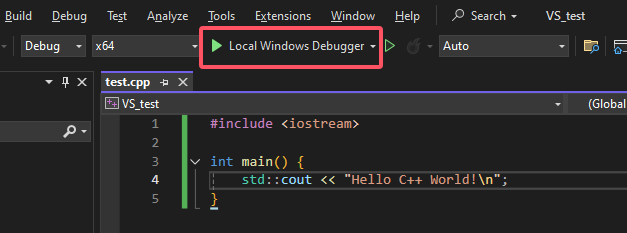
\includegraphics[width=0.50\linewidth]{pic/VS_Build.png}
    \end{figure}
    if you are using Linux or Mac OS, please type \cverb|g++ *.cpp| under the folder your source file locates. You will get a file called \cverb|a.out|. That will be your program and you can run it. 
\end{frame}

\end{document}
